\documentclass[]{article}

% Get better typography
\usepackage[protrusion=true,expansion=true]{microtype}		

% For algorithms
\usepackage[boxruled,linesnumbered,vlined,inoutnumbered]{algorithm2e}
\SetKwInOut{Parameter}{Parameters}

% For basic math, align, fonts, etc.
\usepackage{amsmath}
\usepackage{amsthm}
\usepackage{amssymb}
\usepackage{mathtools}
\usepackage{mathrsfs}
\usepackage{rotating}
\usepackage{gensymb} % For \degree
\usepackage{enumitem} %for enumerating with letters
\usepackage{booktabs}
\usepackage{graphicx}
\usepackage{float}
\usepackage{xcolor}
\usepackage[top=2cm, bottom=2cm, left = 1cm, right = 1cm,columnsep=20pt]{geometry}


\newtheorem{defn}{Definition}[]
\newtheorem{thm}{Theorem}[]
\newtheorem{claim}{Claim}[]
\newtheorem{lemma}{Lemma}[]
\newtheorem{prop}{Property}[]
\newtheorem{ass}{Assumption}[]
\newtheorem{cor}{Corollary}[]

\DeclareMathOperator*{\argmin}{arg\,min}
\DeclareMathOperator*{\argmax}{arg\,max}

\usepackage{courier} % For \texttt{foo} to put foo in Courier (for code / variables)
\usepackage{lipsum} % For dummy text

% For images
\usepackage{graphicx}
\usepackage{subcaption}
\usepackage[space]{grffile} % For spaces in image names

% For bibliography
\usepackage[round]{natbib}

% For color
\usepackage{xcolor}
\definecolor{light-grey}{rgb}{0.95,0.95,0.95}
\definecolor{dark-red}{rgb}{0.4,0.15,0.15}
\definecolor{dark-blue}{rgb}{0,0,0.7}

% For questions and answers
\usepackage[framemethod=tikz]{mdframed}
\newtheorem{question}{Question}
\mdfdefinestyle{que}{
  linecolor=dark-blue,
  backgroundcolor=white!20,
}
\surroundwithmdframed[style=que]{question}
\newtheorem{answer}{Answer}
\mdfdefinestyle{ans}{
  linecolor=dark-red,
  backgroundcolor=white!20
  % , rotatebox
}
\surroundwithmdframed[style=ans]{answer}
\usepackage{environ}
\NewEnviron{Answer}
{%
\noindent
\rotatebox[origin=c]{180}{%
\noindent
\begin{minipage}[t]{\linewidth}
\begin{answer}
\BODY
\end{answer}%
\end{minipage}%
}%
}%

% Only show sections in table of contents and rename
\setcounter{tocdepth}{2}
\renewcommand{\contentsname}{Table of Contents}

% For links (e.g., clicking a reference takes you to the phy)
\usepackage{hyperref}
\hypersetup{
    colorlinks, linkcolor={dark-blue},
    citecolor={dark-blue}, urlcolor={dark-blue}
}

%-------------------------
%	TOGGLE ANSWER VISIBILITY
%-------------------------
\newif\ifHomeworkOneAnswers
\HomeworkOneAnswersfalse
%\HomeworkOneAnswerstrue

%-------------------------
%	BEGIN DOCUMENT / TITLE
%-------------------------

\begin{document}
%-----------------
%	Homework 2
%-----------------
\newpage
\begin{center}
    \begin{Large}
    CMPSCI 687 Homework 2
    \end{Large}
    \\
    Due October 3, 2018, 11:55pm Eastern Time
\end{center}
\addcontentsline{toc}{subsection}{\textbf{Homework 2}}

\noindent {\bf Instructions: } This homework  consists of a programming portion only. Collaboration is not allowed on any part of this assignment. Submissions must be typed (hand written and scanned submissions will not be accepted). You must use \LaTeX. The coding portion of the assignment should be submitted on Gradescope as a .zip file containing your code (see details below). The written response answers should be submitted to Gradescope via a .pdf file and a tagged with the relevant pages. You \textbf{must} use the template we have provided, which is located at the github repository \href{https://github.com/bmetevier/rl-framework-687-public}{here}. You may not use any reinforcement learning or machine learning specific libraries in your code, e.g., TensorFlow or PyTorch (you may use libraries like numpy and matplotlib though). If you are unsure whether you can use a library, ask on Piazza. The automated system will not accept assignments after 11:55pm on October 3. The tex file for this homework can be found \href{https://people.cs.umass.edu/~pthomas/courses/CMPSCI_687_Fall2019/hw2Source.tex}{here}. The number of points for this assignment is 100. 

\section*{Implement Cart-Pole}

In this assignment you will implement the cart-pole domain using the (frictionless) dynamics described by \citet[Equations 23 and 24]{Florian2007}, we provide the expressions below. 
%When implementing cart-pole, the state should include the position of the cart, velocity of the cart, angle of the pole, and angular velocity of the pole. 
You \textbf{must} use a forward Euler approximation of the dynamics. If the cart hits the boundary of the track, the pole falls below a fail angle, or the time limit is exceeded, then terminate the episode.
%
\textbf{You may not use existing RL code for this problem---you must implement the agent and environment entirely on your own and using the class template.} 

The Cart-pole environments consists of two interacting bodies: a cart with position $x$ and velocity $\dot x$, and a pole with angle $\theta$ and angular velocity $\dot \theta$. 
%
An expression for the pole's angular acceleration is 
%
\begin{equation}
    \ddot \theta = \frac{g \sin{\theta} + \cos{\theta}\left( \frac{-F-m_p l \dot \theta^2 \sin \theta}{m_c + m_p}\right )}{l \left ( \frac{4}{3} - \frac{m_p \cos^2{\theta}}{m_c + m_p}\right )},
\end{equation}
%
where $g$ is the acceleration due to gravity, $F$ is the force applied to the cart, $m_p$ is the mass of the pole, $m_c$ is the mass of the cart, and $l$ is half the length of the pole. 
%
An expression for acceleration of the cart is 
%
\begin{equation}
    \ddot x = \frac{F + m_p l (\dot \theta^2 \sin{\theta} - \ddot \theta \cos{\theta})}{m_c + m_p}.    
\end{equation}
%
The system state is described by the state vector $\mathbf{x} \coloneqq [x, v, \theta, \omega ]$, where $v = \dot x$ and $\omega = \dot \theta$. 

The state space equations of motion are:
%
\begin{align}
    \dot x_{t} = &\ v_t \\
    \dot v_{t} = &\ \frac{F + m_p l (\dot \theta_t^2 \sin{\theta_t} - \dot \omega_t \cos{\theta_t})}{m_c + m_p} \\
    \dot \theta_t = &\ \omega_t \\
    \dot \omega_t = &\ \frac{g \sin{\theta_t} + \cos{\theta_t}\left( \frac{-F-m_p l \omega_t^2 \sin \theta_t}{m_c + m_p}\right )}{l \left ( \frac{4}{3} - \frac{m_p \cos^2{\theta_t}}{m_c + m_p}\right )}.
\end{align}
%
Using the Euler approximation the system evolves as:
\begin{equation}
    \mathbf{x}_{t+1} = \mathbf{x}_t + \Delta t \dot {\mathbf{x}}_t,
\end{equation}
where $\dot {\mathbf{x}}_t = [\dot x_t, \dot v_t, \dot \theta_t, \dot \omega_t]$ and $\Delta t$ is the time in seconds between updates. 
%
In this environment, an agent's action specifies a force $F \in [-F_\text{mag}, F_\text{mag}]$ on the cart. Traditionally, in RL, the cart pole environment is specified with two discrete actions, where $a_0 = -F_\text{mag}$ and $a_1 = F_\text{mag}$. You must use this action space in creating the environment.

Use the following values for the cart-pole constants:
\begin{itemize}
    \item Fail angle $= \pi/12$. (If it exceeds this value or its negative, the episode ends in failure.)
    \item Cart boundaries are at $x=-3m$ and $x=3m$.
    \item Max motor force magnitude $F_\text{mag} = 10.0$ (force on cart in Newtons).
    \item Gravitational constant $g$ is $9.8$.
    \item Cart mass $m_c = 1.0 \text{ kg}$.
    \item Pole mass $m_p = 0.1 \text{ kg}$.
    \item Pole half-length $l = 0.5m$.
    \item $\Delta t = 0.02\text{ seconds}$ (time step).
    \item Max time before end of episode $= 20\text{ seconds}$.
\end{itemize}

\section*{Genetic Algorithms}
Genetic algorithms (GAs) are a family of biologically inspired BBO algorithms that are empirically competitive with deep reinforcement learning methods \citep{such2017deep}. Intuitively, the GA starts with a population of \emph{candidate solutions} (in our case, parameterized policies $\theta$) and iteratively modifies, or evolves, the population. We call the number of iterations over which a population is evolved the number of \emph{generations}. 

At every generation, the GA uses three main methods, called \emph{genetic operators}, to create the next generation. These genetic operators are known as parent selection, mutation operators, and crossover operators. \emph{Parent selection} chooses which candidate solutions in the current generation will be used as parents for creating children in the next generation.  \emph{Mutation operators} apply random changes to parents to create children for the next generation. \emph{Crossover operators} combine two or more parents to create children for the next generation.

Example pseudocode for a simple GA is below. Pseudocode for the functions \texttt{get\_parents} and \texttt{get\_children} are purposefully not provided. At each generation, every candidate solution, $\theta_i$, in the population, $P=\{\theta_i\}_{i=0}^K$, is evaluated and a \emph{fitness score} for $\theta_i$ is produced. The top $K_p$ candidate solutions are then chosen to become parents of the next generation (this parent selection method is known as truncation selection). Children are created by selecting a parent uniformly at random to mutate by applying additive Gaussian noise to the parent: $\theta_{\text{child}} = \theta_{\text{parent}} + \alpha\epsilon$, where $\epsilon \sim \mathcal N(0,1)$ and $\alpha$ is a hyperparameter. $K_e$ candidate solutions in the new generation are unmodified copies of the top $K_e$ candidate solutions from the previous generation. This is known as \emph{elitism}. 
\\
\begin{algorithm}[H]
    \For{$g=1$ \KwTo $G$}{
        \For{$k=1$ \KwTo $K$}{
            $\hat J_k = \texttt{evaluate}(\theta_k, N)$\;
        }
        $\texttt{sorted} = \texttt{sort}((\theta_1,\hat J_1), (\theta_2,\hat J_2),\dotsc, (\theta_K, \hat J_K), \text{descending})$\;
        %
        $\texttt{parents} =  \texttt{get\_parents}(K_p, \texttt{sorted})$\;
        %
        $\texttt{next\_gen} = \texttt{sorted}[1:K_e].\texttt{append}(\texttt{get\_children}(\alpha, \texttt{parents}))$\;
    }
\caption{\texttt{Genetic Algorithm} (GA) for Policy Search.\newline
\textbf{Input:}
\newline \textbf{1)} Number of generations, $G \in \mathbb N_{>1}$ [for example, $G=300$]
\newline \textbf{2)} Initial population, $P = \{\theta_i\}_{i=0}^K$
\newline \textbf{3)} Population size, $K \in \mathbb N_{>1}$ [for example, $K=20$]
\newline \textbf{4)} Truncation index, $K_p \in \mathbb N_{>0}$, where $K_p < K$ [for example, $K_p=10$]
\newline \textbf{5)} Elite population, $K_e \in \mathbb N_{>0}$, where $K_e < K$ [for example, $K_e=10$]
\newline \textbf{6)} Number of episodes to sample per policy, $N \in \mathbb N_{>0}$ [for example, $N=10$]
\newline \textbf{7)} Learning parameter $\alpha \in \mathbb R$ [for example, $\alpha=2.5$]}
\label{alg:crossEntropy}
\end{algorithm}

\begin{algorithm}[H]
    Run the parameterized policy using policy parameters $\theta$ for $N$ episodes\;
    Compute the resulting $N$ returns, $G^1,G^2,\dotsc,G^N$, where
    $
    G^i = \sum_{t=0}^\infty R_t^i.
    $\;
    Return $\frac{1}{N}\sum_{i=1}^N G^i$\;
\caption{\texttt{evaluate}\newline
\textbf{Input:}
\newline \textbf{1)} Policy parameter vector, $\theta \in \mathbb R^n$
\newline \textbf{2)} Number of episodes to sample, $N \in \mathbb N_{>0}$ [for example, $N=10$]}
\label{alg:evaluate}
\end{algorithm}
\textbf{Note} that we do not provide pseudocode for the \texttt{get\_parents} and \texttt{get\_children} methods. It will be up to you to define these methods.  

\section*{Problems}
Six questions ask for a plot. You must report two plots: one for cart-pole and one for 687-Gridworld, where each of these two plots has a curve corresponding to the cross-entropy method, a curve corresponding to the GA method, and a curve corresponding to first-choice hill-climbing. In the coding problems your solutions will be graded via an autograder on Gradescope. To submit assignments you must zip the rl687 folder and its structure must be the same as the template. You must use the same files provided in the template and fill in the missing function bodies. Correct solutions can be fit within the provided files, but you can create additional files as necessary for the assignment. However, if any errors occur in using them the questions will be marked as zero. The functions will need to match our outputs exactly so pay attention to types (we use np.float64 and np.int for arrays, int, float, and bool else where). The autograder will give results before the assignment is due so you can check your implementations for correctness. 
\\\\
\noindent \textbf{Coding Problems:}

\begin{enumerate}
    
    \item{(15 Points) Implement the cart-pole environment as specified above.}
    
    \item{(5 Points) Implement the tabular softmax policy.}
    
    \item{(10 Points) Implement the cross-entropy method as described in the class notes.}
    
    \item{(10 Points) Implement the First-choice hill-climbing algorithm as described in the class notes.}
    
    \item{(10 Points) Implement the GA algorithm described earlier in this assignment.}
\end{enumerate}

\noindent\textbf{Written Response:}

\begin{enumerate}
    \item (7.5 Points) Apply the CEM algorithm to the More-Watery 687-Gridworld. Use a tabular softmax policy. Search the space of hyperparameters for hyperparameters that work well. Report how you searched the hyperparameters, what hyperparameters you found worked best, and present a learning curve plot using these hyperparameters, as described in class. This plot may be over any number of episodes, but should show convergence to a nearly optimal policy. The plot should average over at least $500$ trials and should include standard deviation error bars. 

	{
		\color{blue}
		Ans. For the Cross Entropy Method Algorithm on the More-Watery 687-Gridworld domain, I have searched a huge space of hyperparameters. My final set of hyperparameters that work best are: population size ($K$) = 10, elite population size ($K_e$) = 5, numeric stability parameter($\epsilon$) = 4.0, sigma = 1.0, number of episodes (numEpisodes) = 20, number of trials (numTrials) = 5, and number of iterations (numIterations) = 50. Additionally, each episode was run for a maximum of 200 time steps. I started with numTrials = 5 and sigma = 1.0  which I did not change throughout my journey of searching for the best hyperparameters. Additionally,  I started with a huge number of iterations (numIterations = 500), number of episodes (numEpisodes = 500),  $K$ = 20, $K_e$ = 10, and $\epsilon$ = 0.0001. When I noticed that the Expected Return towards the end of the trials were converging to 0 for most trials, I understood that the agent was stuck in a bad space of hyperparameters. So, I started increasing $\epsilon$ on a logarithmic scale. As I started noticing improvement on the convergence of the Expected Return with higher values of $\epsilon$, I started decreasing the number of iterations roughly on a linear scale and number of episodes roughly on a logarithmic scale, to decrease the run-time of the algorithm. Thus, when I noticed nice performance of the curve (convergence to an Expected Return of 3 for a large number of episodes at the end of the curve), I settled at $\epsilon$ = 4.0, numIterations = 50, and numEpisodes = 20. To reduce the run-time of the algorithm even further while retaining the convergence to an Expected Return of 3, I noticed that I could reduce $K$ and $K_e$ slightly. Thus, I decreased $K$ to 10 and $K_e$ to 5 while retaining the curve to converge at an Expected Return of 3. Then, I plotted the curve a final time with  $K$ = 10, $K_e$ = 5, $\epsilon$ = 4.0, sigma = 1.0, numEpisodes = 20, numTrials = 5, and numIterations = 50, which gave the curve that converges to an Expected Return of 3.
		
		\begin{figure}[H]
		    \centering
		    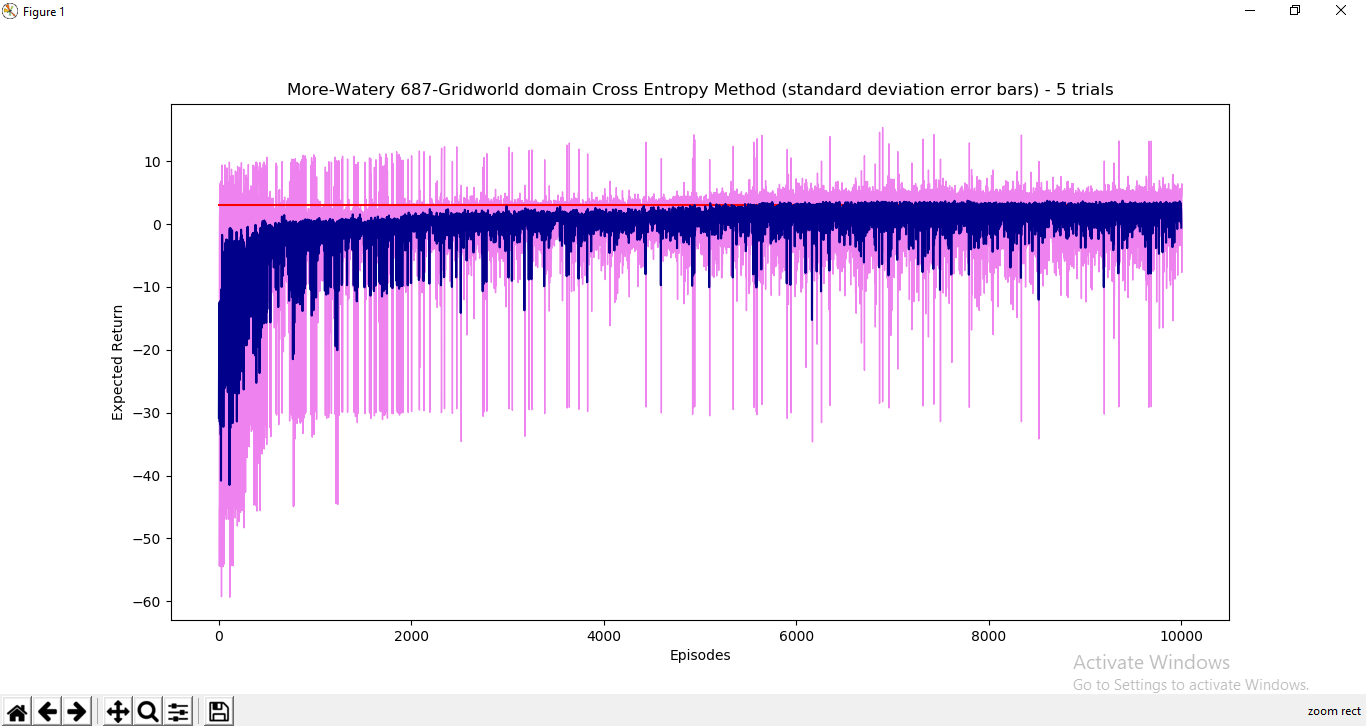
\includegraphics[width=1.0\textwidth]{CEM Gridworld Plot.png}
		    \caption{Cross Entropy Method algorithm for More-Watery 687-Gridworld domain using 5 trials. The red line is  at Expected Return = 3. The Standard Deviation is represented using violet color and the mean is represented using dark blue color.}
		    \label{fig: Cross Entropy Method algorithm for More-Watery 687-Gridworld}
		\end{figure}

	}
    
    \item (7.5 Points) Repeat the previous question, but using first-choice hill-climbing on the More-Watery 687-Gridworld domain. Report the same quantities.

	{
		\color{blue}
		Ans . For the First Choice Hill Climbing Algorithm on the More-Watery 687-Gridworld domain, I have searched a huge space of hyperparameters. My final set of hyperparameters that work best are: exploration parameter ($\sigma$) = 1.0, number of episodes (numEpisodes) = 200, number of trials (numTrials) = 50, and number of iterations (numIterations) = 200. Additionally, each episode was run for a maximum of 200 time steps. I started with numTrials = 50 and $\sigma$ = 1.0  which I did not change throughout my journey of searching for the best hyperparameters. Additionally,  I started with a huge number of iterations (numIterations = 500) and number of episodes (numEpisodes = 500). When I noticed that the Expected Return towards the end of the trials for many episodes were converging to above 0 for most trials, I understood that the agent could also perform the same way with fewer number of episodes and fewer number of iterations. So, I started decreasing the number of iterations and the number of episodes on roughly linear scales , to decrease the run-time of the algorithm. Thus, when I noticed nice performance of the curve (convergence to an Expected Return of above 0 for a large number of episodes at the end of the curve), I settled at numIterations = 200 and numEpisodes = 200. Then, I plotted the curve a final time with  exploration parameter ($\sigma$) = 1.0, number of episodes (numEpisodes) = 200, number of trials (numTrials) = 50, and number of iterations (numIterations) = 200, which gave the curve that converges to an Expected Return of above 0.
		
		\begin{figure}[H]
		    \centering
		    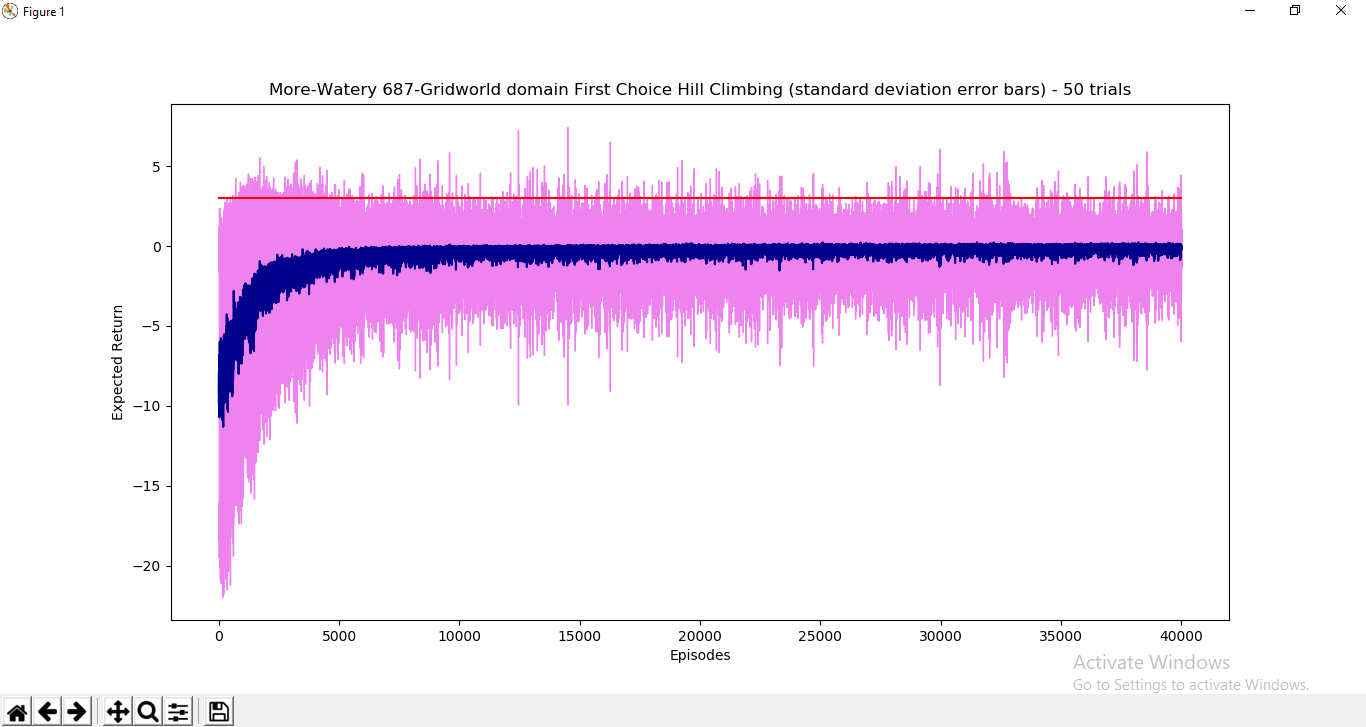
\includegraphics[width=1.0\textwidth]{FCHC Gridworld Plot.png}
		    \caption{First Choice Hill Climbing Algorithm for More-Watery 687-Gridworld using 50 trials. The red line is  at Expected Return = 3. The Standard Deviation is represented using voilet color and the mean is represented using dark blue color.}
		    \label{fig: First Choice Hill Climbing Algorithm for More-Watery 687-Gridworld}
		\end{figure}

	}
    
    \item (7.5 Points) Repeat the previous question, but using the GA (as described earlier in this assignment) on the More-Watery 687-Gridworld domain. Report the same quantities.

	{
		\color{blue}
		Ans . For the Genetic Algorithm on the More-Watery 687-Gridworld domain, I have searched a huge space of hyperparameters. My final set of hyperparameters that work best are: population size ($K$) = 40, elite population size ($K_e$) = 20, learning parameter  ($\alpha$) = 3.0, truncation index ($K_p$) = 30, number of episodes (numEpisodes) = 20, number of trials (numTrials) = 50, and number of generations ($G$) = 100. Additionally, each episode was run for a maximum of 200 time steps. I started with numTrials = 50, $K$ = 40, $K_e$ = 10, $K_p$ = 30, and $\alpha$ = 3.0  which I did not change throughout my journey of searching for the best hyperparameters. Additionally,  I started with a huge number of episodes (numEpisodes = 200) and  $G$ = 200. When I noticed that the Expected Return towards the end of the trials were converging to an Expected Return of 3 for most trials, I understood that decreasing the number of iterations and the number of episodes would still yield a curve that converged to an Expected Return of 3. So, I started decreasing numEpisodes and $G$ on roughly linear scales, to decrease the run-time of the algorithm. Thus, when I noticed nice performance of the curve (convergence to an Expected Return of 3 for a large number of episodes at the end of the curve), I settled at $numEpisodes$ = 20 and $G$ = 100. Then, I plotted the curve a final time with  population size ($K$) = 40, elite population size ($K_e$) = 20, learning parameter  ($\alpha$) = 3.0, truncation index ($K_p$) = 30, number of episodes (numEpisodes) = 20, number of trials (numTrials) = 50, and number of generations ($G$) = 100, which gave the curve that converges to an Expected Return of 3.
		
		\begin{figure}[H]
		    \centering
		    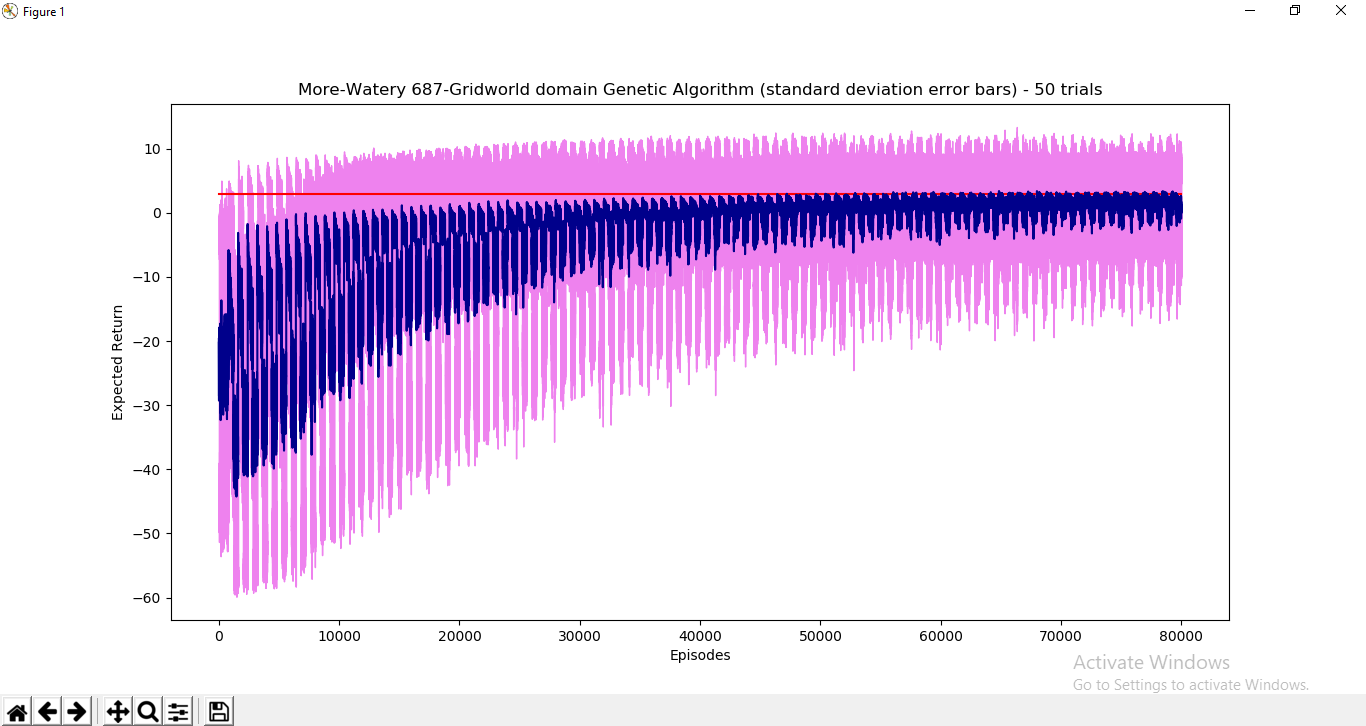
\includegraphics[width=1.0\textwidth]{GA Gridworld Plot.png}
		    \caption{Genetic Algorithm for More-Watery 687-Gridworld using 50 trials. The red line is  at Expected Return = 3. The Standard Deviation is represented using violet color and the mean is represented using dark blue color.}
		    \label{fig: Genetic Algorithm for More-Watery 687-Gridworld}
		\end{figure}

	}
    
    \item (7.5 Points) Repeat the previous question, but using the cross-entropy method on the cart-pole domain. Notice that the state is not discrete, and so you cannot directly apply a tabular softmax policy. It is up to you to create a representation for the policy for this problem. Consider using the softmax action selection using linear function approximation as described in the notes. For descriptions of common choices of $\phi$, see the work of \cite{Konidaris2011}. Report the same quantities, as well as how you parameterized the policy. 

	{
		\color{blue}
		Ans. For the Cross Entropy Method Algorithm on the Cartpole domain, I have searched a huge space of hyperparameters. My final set of hyperparameters that work best are: population size ($K$) = 10, elite population size ($K_e$) = 5, numeric stability parameter($\epsilon$) = 4.0, sigma = 1.0, number of episodes (numEpisodes) = 20, number of trials (numTrials) = 5, linear function approximation parameter ($k$) = 2, and number of iterations (numIterations) = 40. Additionally, each episode was run for a maximum of 1000 time steps. I started with numTrials = 5, $k$ = 2, and sigma = 1.0  which I did not change throughout my journey of searching for the best hyperparameters. Additionally,  I started with a huge number of iterations (numIterations = 1000), number of episodes (numEpisodes = 1000),  $K$ = 20, $K_e$ = 10, and $\epsilon$ = 0.0001. When I noticed that the Expected Return towards the end of the trials were not converging to an Expected Return of 1000 for most trials, I understood that the agent was stuck in a bad space of hyperparameters. So, I started increasing $\epsilon$ on a logarithmic scale. As I started noticing improvement on the convergence of the Expected Return with higher values $\epsilon$, I started decreasing the number of iterations and the number of episodes roughly on a logarithmic scale, to decrease the run-time of the algorithm. Thus, when I noticed nice performance of the curve (convergence to an Expected Return of 1000 for a large number of episodes at the end of the curve), I settled at $\epsilon$ = 4.0, numIterations = 40, and numEpisodes = 20. To reduce the run-time of the algorithm even further while retaining the convergence to 1000, I noticed that I could reduce $K$ and $K_e$ slightly. Thus, I decreased $K$ to 10 and $K_e$ to 5 while retaining the curve to converge at an expected return of 1000. Then, I plotted the curve a final time with  $K$ = 10, $K_e$ = 5, $\epsilon$ = 4.0, sigma = 1.0, numEpisodes = 20, numTrials = 5, $k$ = 2, and numIterations = 40, which gave the curve that converges to an Expected Return of 1000.
		
		\begin{figure}[H]
		    \centering
		    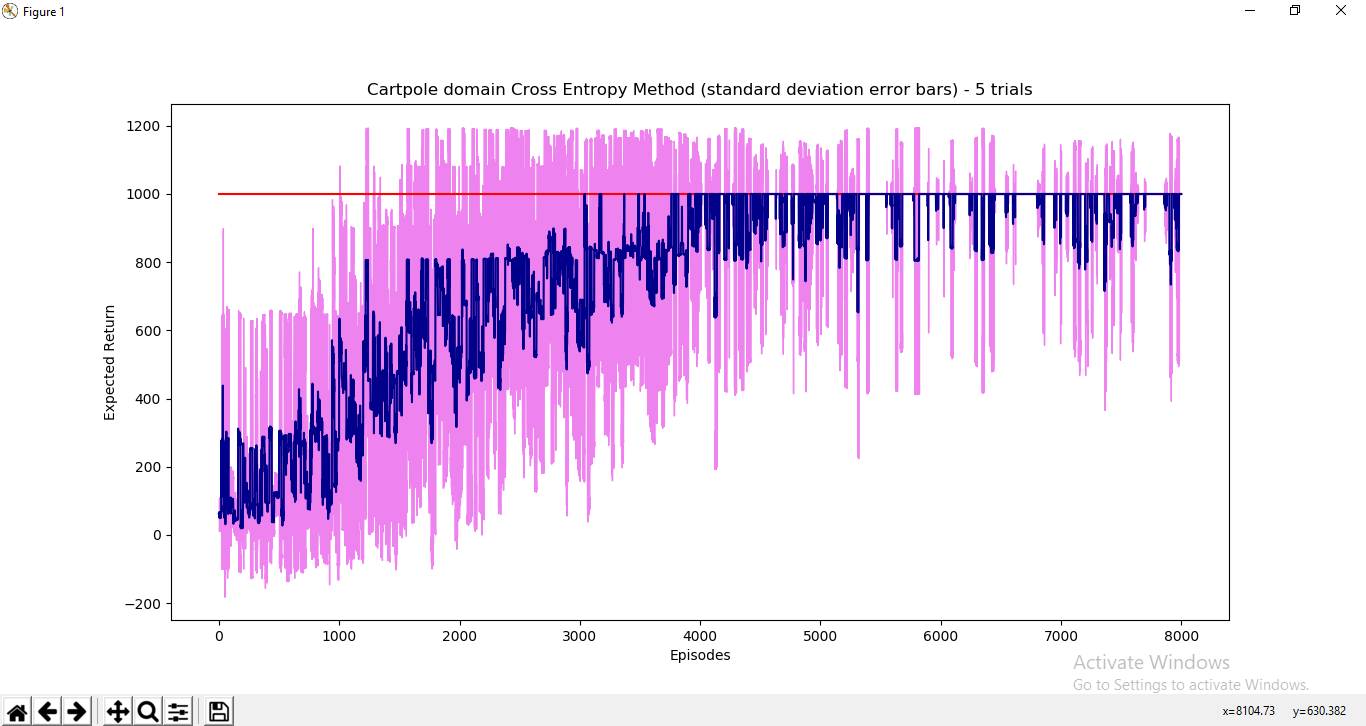
\includegraphics[width=1.0\textwidth]{CEM Cartpole Plot.png}
		    \caption{Cross Entropy Method algorithm for Cartpole domain using 5 trials. The red line is  at Expected Return = 1000. The Standard Deviation is represented using violet color and the mean is represented using dark blue color.}
		    \label{fig: Cross Entropy Method algorithm for Cartpole}
		\end{figure}

	}
    
    \item (7.5 Points) Repeat the previous question, but using first-choice hill-climbing (as described in class) on the cart-pole domain. Report the same quantities and how the policy was parameterized. 

	{
		\color{blue}
		Ans . For the First Choice Hill Climbing Algorithm on the Cartpole domain, I have searched a huge space of hyperparameters. My final set of hyperparameters that work best are: exploration parameter ($\sigma$) = 1.0, number of episodes (numEpisodes) = 100, number of trials (numTrials) = 50, linear function approximation parameter ($k$) = 2, and number of iterations (numIterations) = 50. Additionally, each episode was run for a maximum of 1000 time steps. I started with numTrials = 50, $k$ = 2, and $\sigma$ = 1.0  which I did not change throughout my journey of searching for the best hyperparameters. Additionally,  I started with a huge number of iterations (numIterations = 500) and number of episodes (numEpisodes = 500). When I noticed that these values for numIterations and numEpisodes were computationally really expensive for 50 trails and that it was taking a really long time to output the plot, I started checking the values of the expected return it was outputing as the agent was trying different episodes. I noticed that decreasing numIterations and numEpisodes roughly on a linear scale did not affect the expected returns towards the end of the trials much, so I started decreasing numIterations and numEpisodes on roughly linear scales to decrease the run-time of the algorithm. Thus, when I noticed nice performance of the curve (convergence to an Expected Return of above 700 for a large number of episodes at the end of the curve), I settled at numIterations = 50 and numEpisodes = 100. Then, I plotted the curve a final time with exploration parameter ($\sigma$) = 1.0, number of episodes (numEpisodes) = 100, number of trials (numTrials) = 50, linear function approximation parameter ($k$) = 2, and number of iterations (numIterations) = 50, which gave the curve that converges to an Expected Return of above 700.
		
		\begin{figure}[H]
		    \centering
		    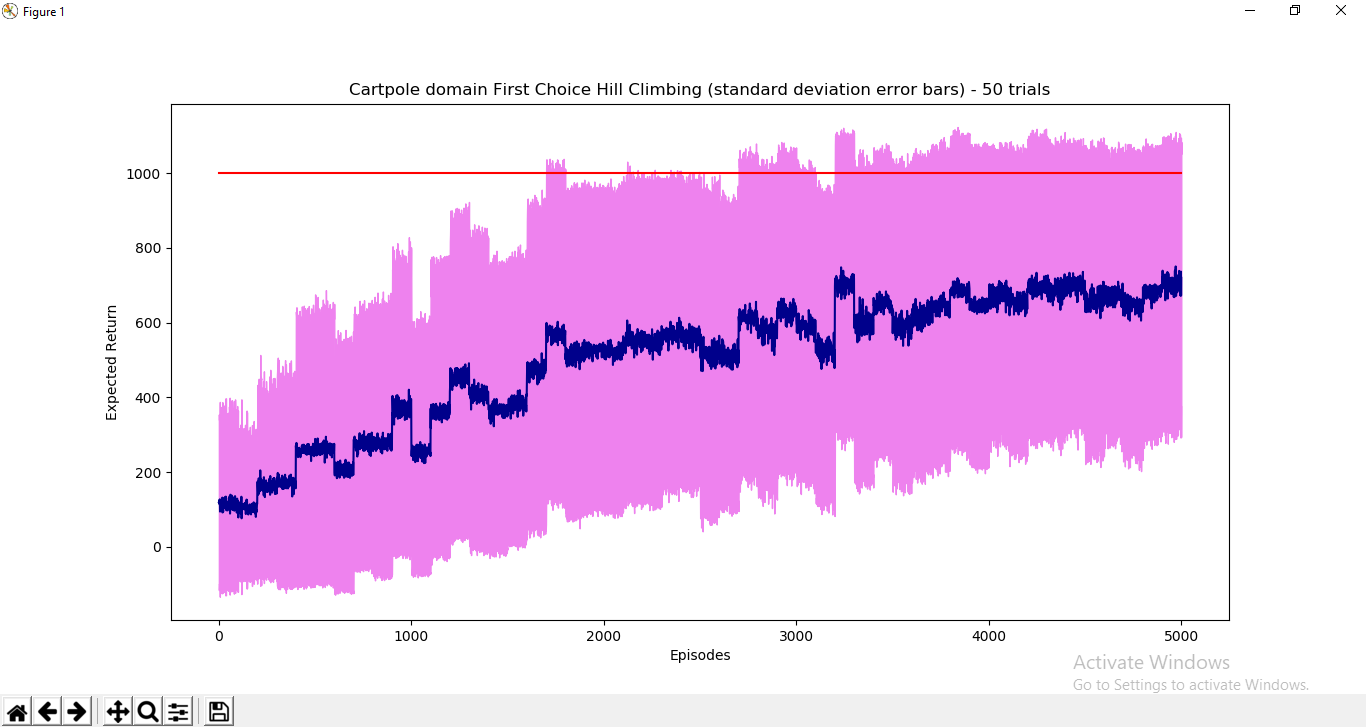
\includegraphics[width=1.0\textwidth]{FCHC Cartpole Plot.png}
		    \caption{First Choice Hill Climbing Algorithm for Cartpole using 50 trials. The red line is  at Expected Return = 1000. The Standard Deviation is represented using pink color and the mean is represented using dark blue color.}
		    \label{fig: First Choice Hill Climbing Algorithm for Cartpole}
		\end{figure}

	}
    
    
    \item (7.5 Points) Repeat the previous question, but using the GA (as described earlier in this homework) on the cart-pole domain. Report the same quantities and how the policy was parameterized. 

	{
		\color{blue}
		Ans . For the Genetic Algorithm on the Cartpole domain, I have searched a huge space of hyperparameters. My final set of hyperparameters that work best are: population size ($K$) = 20, elite population size ($K_e$) = 5, learning parameter  ($\alpha$) = 2.5, truncation index ($K_p$) = 10, number of episodes (numEpisodes) = 5, number of trials (numTrials) = 50, linear function approximation parameter ($k$) = 2, and number of generations ($G$) = 20. Additionally, each episode was run for a maximum of 1000 time steps. I started with numTrials = 50, $K$ = 20, $K_e$ = 5, $K_p$ = 10, linear function approximation parameter ($k$) = 2, and $\alpha$ = 2.5  which I did not change throughout my journey of searching for the best hyperparameters. Additionally,  I started with a huge number of episodes (numEpisodes) = 200 and  $G$ = 200. When I noticed that the Expected Return towards the end of the trials were converging to 1000 for most trials, I understood that decreasing the number of iterations and the number of episodes would still yield a curve that converged to an Expected Return of 1000. So, I started decreasing numEpisodes and $G$ roughly on linear scales, to decrease the run-time of the algorithm. Thus, when I noticed nice performance of the curve (convergence to an Expected Return of 1000 for a large number of episodes at the end of the curve), I settled at numEpisodes = 5 and $G$ = 20. Then, I plotted the curve a final time with  population size ($K$) = 20, elite population size ($K_e$) = 5, learning parameter  ($\alpha$) = 2.5, truncation index ($K_p$) = 10, number of episodes (numEpisodes) = 5, number of trials (numTrials) = 50, linear function approximation parameter ($k$) = 2, and number of generations ($G$) = 20, which gave the curve that converges to an Expected Return of 1000.
		
		\begin{figure}[H]
		    \centering
		    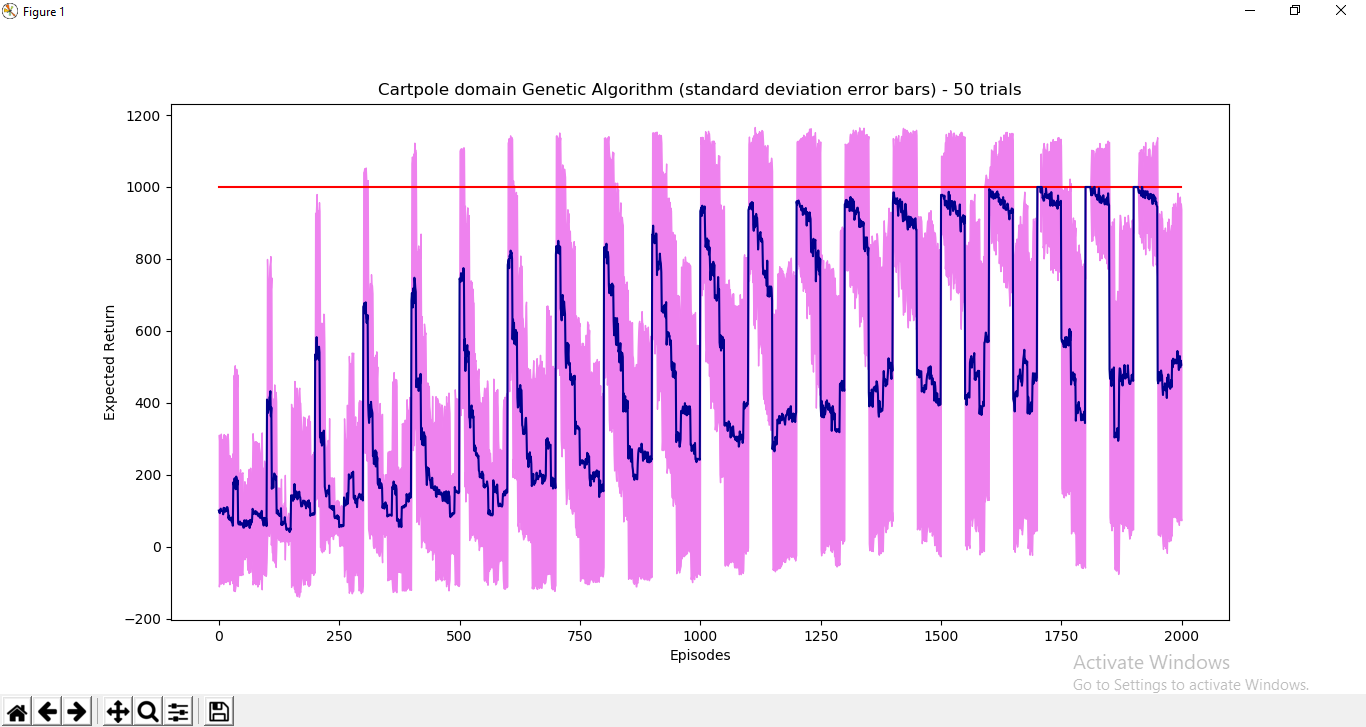
\includegraphics[width=1.0\textwidth]{GA Cartpole Plot.png}
		    \caption{Genetic Algorithm for Cartpole domain using 50 trials. The red line is  at Expected Return = 1000. The Standard Deviation is represented using violet color and the mean is represented using dark blue color.}
		    \label{fig: Genetic Algorithm for Cartpole}
		\end{figure}

	}
    
    \item (5 Points) Reflect on this problem. Was it easier or harder than you expected to get these methods working? In the previous assignment you hypothesized how long it would take an agent to solve the More-Watery 687-Gridworld problem. Did it take more or fewer episodes than you expected? Why do you think this happened?

	{
		\color{blue}
		Ans . It was significantly harder than expected to get these methods working. The implementations of the algorithms themselves were easy, but tuning the hyperparameters to converge to reasonably nice values of Expected Returns were challenging. In other words, it was challenging to provide nice hyperparameters which would take the agent to  near-optimal search spaces to yield the best expected returns. In Assignment 1, I hypothesized that I would expect it to take 279,841 ($23^4$) number of episodes for an agent to find near-optimal policies for the More-Watery 687-Gridworld domain. This was because the gridworld has 23 states (without obstacles) and 4 actions that it can taken at each state. So, in my opinion, it should have taken roughly 279,841 ($23^4$) number of episodes to find near-optimal policies if the agent were to select actions in a uniformly random manner. Although, it took significantly fewer number of episodes than what I thought before. This is because the agent does not select actions in a uniformly random manner for each episode. It learns to optimize the policy as the training proceeds, so it starts biasing certain actions at certain states. Thus, it increases the probabilities of taking actions at states that would yield better expected returns. This leads to the agent reaching near-optimal policies much faster when compared to picking actions in a uniformly random manner each time in which no learning takes place. In sum, in my opinion, it is this training phase that optimizes the policy table of the agent to choose actions that yield better expected returns, that makes the agent take significantly fewer number of episodes to reach near-optimal policies.

	}
\end{enumerate}

\bibliography{mybib}
\bibliographystyle{abbrvnat}	% Uses author initials (requires abbrvnat.bst)

\end{document}